\chapter{实现行人控制系统}

\section{系统架构与设计初步}

本行人控制系统基于 Carla 仿真平台用 Python 编程语言及其 Carla API 实现核心功能,目标是在虚拟环境模拟行人运动控制,通过调节移动、检测周围障碍物及避障等完成复杂导航任务,初步设计 “单向行走”“过马路”“来回行走” 三类基础行为后期可扩展为 “随机漫步”“群体避障” 等高级策略。系统架构由环境设置与初始化、行人控制、碰撞检测与避障、用户输入与交互模块构成,环境设置与初始化模块基于 Carla 的 Town1 地图加载城市道路等元素并随机分布静态和动态障碍物增强场景多样性与鲁棒性,为行人挂载 RGB 摄像头和碰撞传感器设置不同采样频率与视野范围提供视觉感知和避障算法数据,行人控制模块用 Carla 的 WalkerControl 类精确调节行人速度、方向和避障行为实现精确运动控制,碰撞检测与避障模块依赖 Carla 传感器系统让行人实时感知障碍物并避让,通过实时检测动态调整路径避碰,用户输入与交互模块为实验操作提供便利,实现键盘控制行人移动使用户与系统交互更直观便捷。由此设计出了如下图 \ref{fig:system_architecture}所示的行人控制系统架构。

\begin{figure}[H]
    \centering
    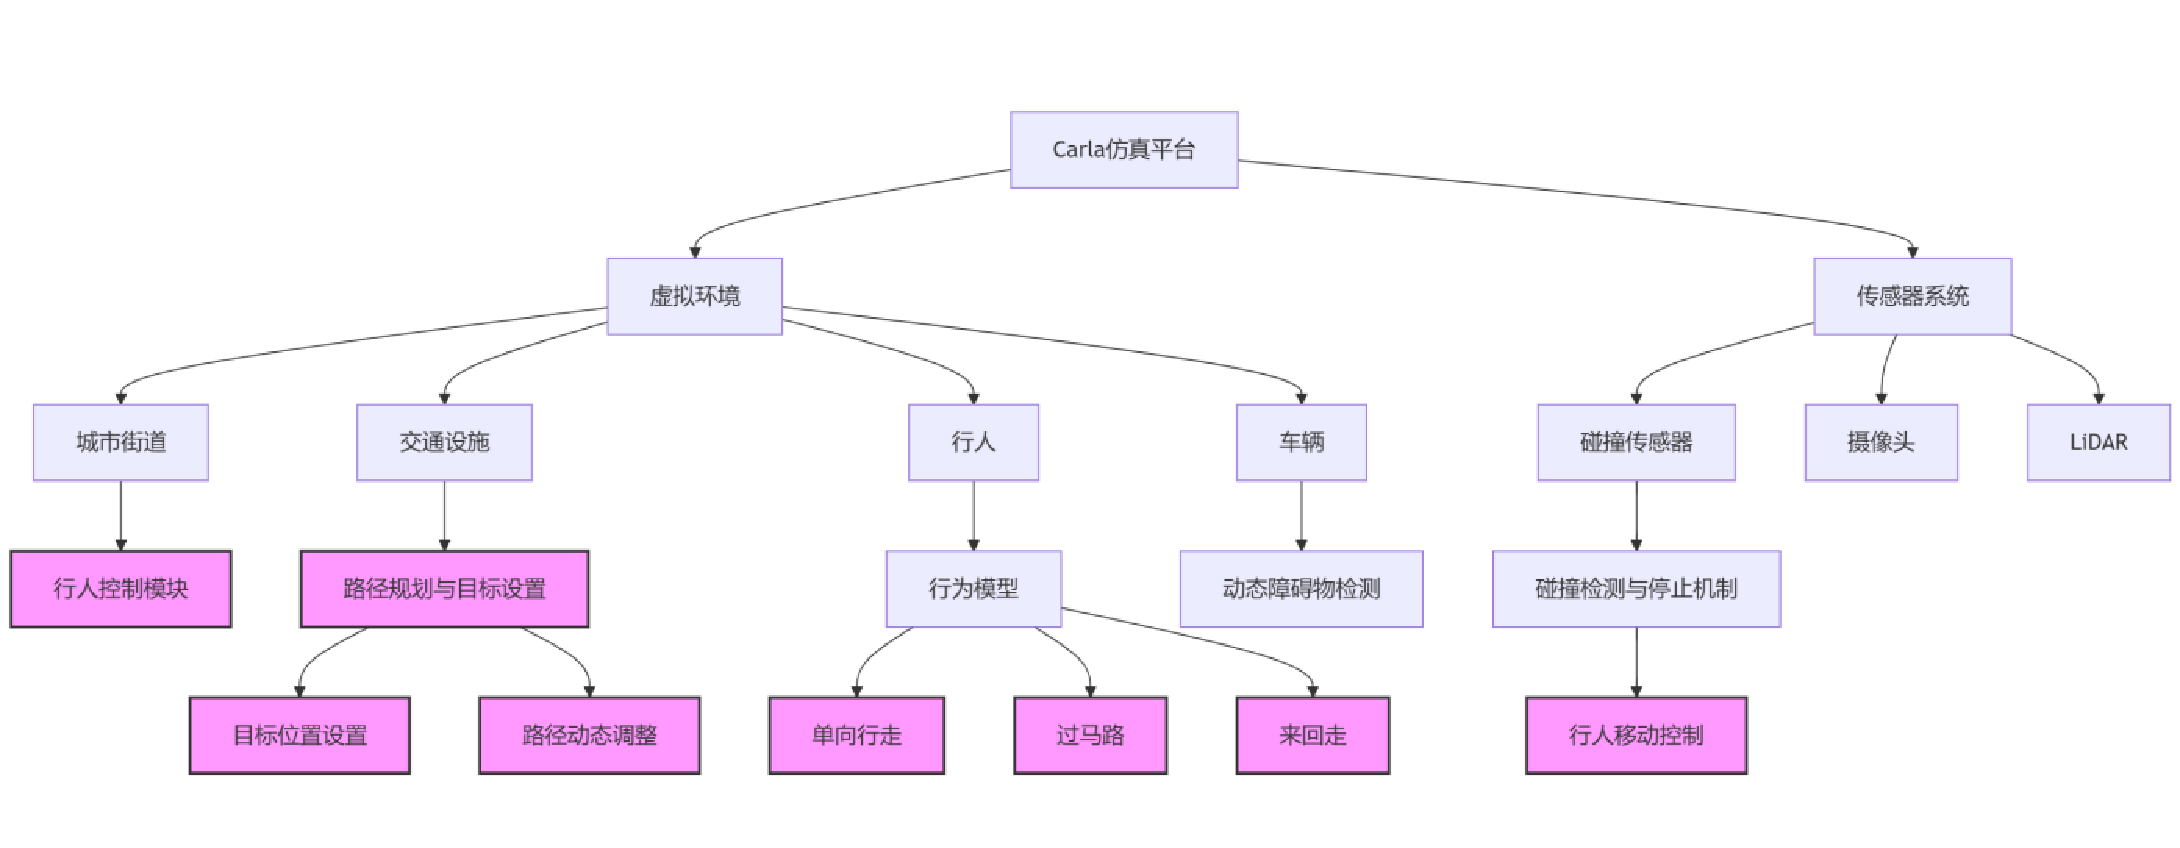
\includegraphics[width=0.8\textwidth]{images/system_architecture.pdf}
    \caption{行人控制系统架构示意图}
    \label{fig:system_architecture}
\end{figure}

\section{行人骨骼控制}

在行人行为研究中准确获取骨骼姿态信息是实现行为理解与决策的关键,结合 Carla 平台 AI 行人生成功能与自定义脚本设计可实现模拟环境中行人骨骼数据的完整采集处理及后续深度学习模型训练验证,为训练行人识别建筑物道路汽车人行道及过马路行人以保障安全,Carla 模拟器通过人工智能控制的行人填充模拟和训练数据,人体姿态估计在自动驾驶安全人群控制及机器人等多个计算机视觉应用中是重要因素。

Carla 的 API 支持从模拟行人获取真实骨架,该骨架由含根节点或顶点及定义骨骼姿势向量的一组骨骼组成,如下图 \ref{fig:pedestrian_skeleton}所示,这些骨骼控制模拟行人四肢和身体运动,通过收集各骨骼集合可构建虚拟人姿势模型,该模型能与神经网络估计的姿势模型比较甚至用于训练神经网络进行姿势估计,通过 AI 控制器生成行人并恢复其骨骼真实三维坐标,将这些骨骼投影到相机传感器捕获的二维图像上,可在 Carla 模拟器中为人体姿势估计框架设置训练和验证,保证骨骼数据采集的完整性和精度能为后续基于 Carla 环境的行人姿态估计与行为预测模型提供坚实数据基础。

\begin{figure}[H]
    \centering
    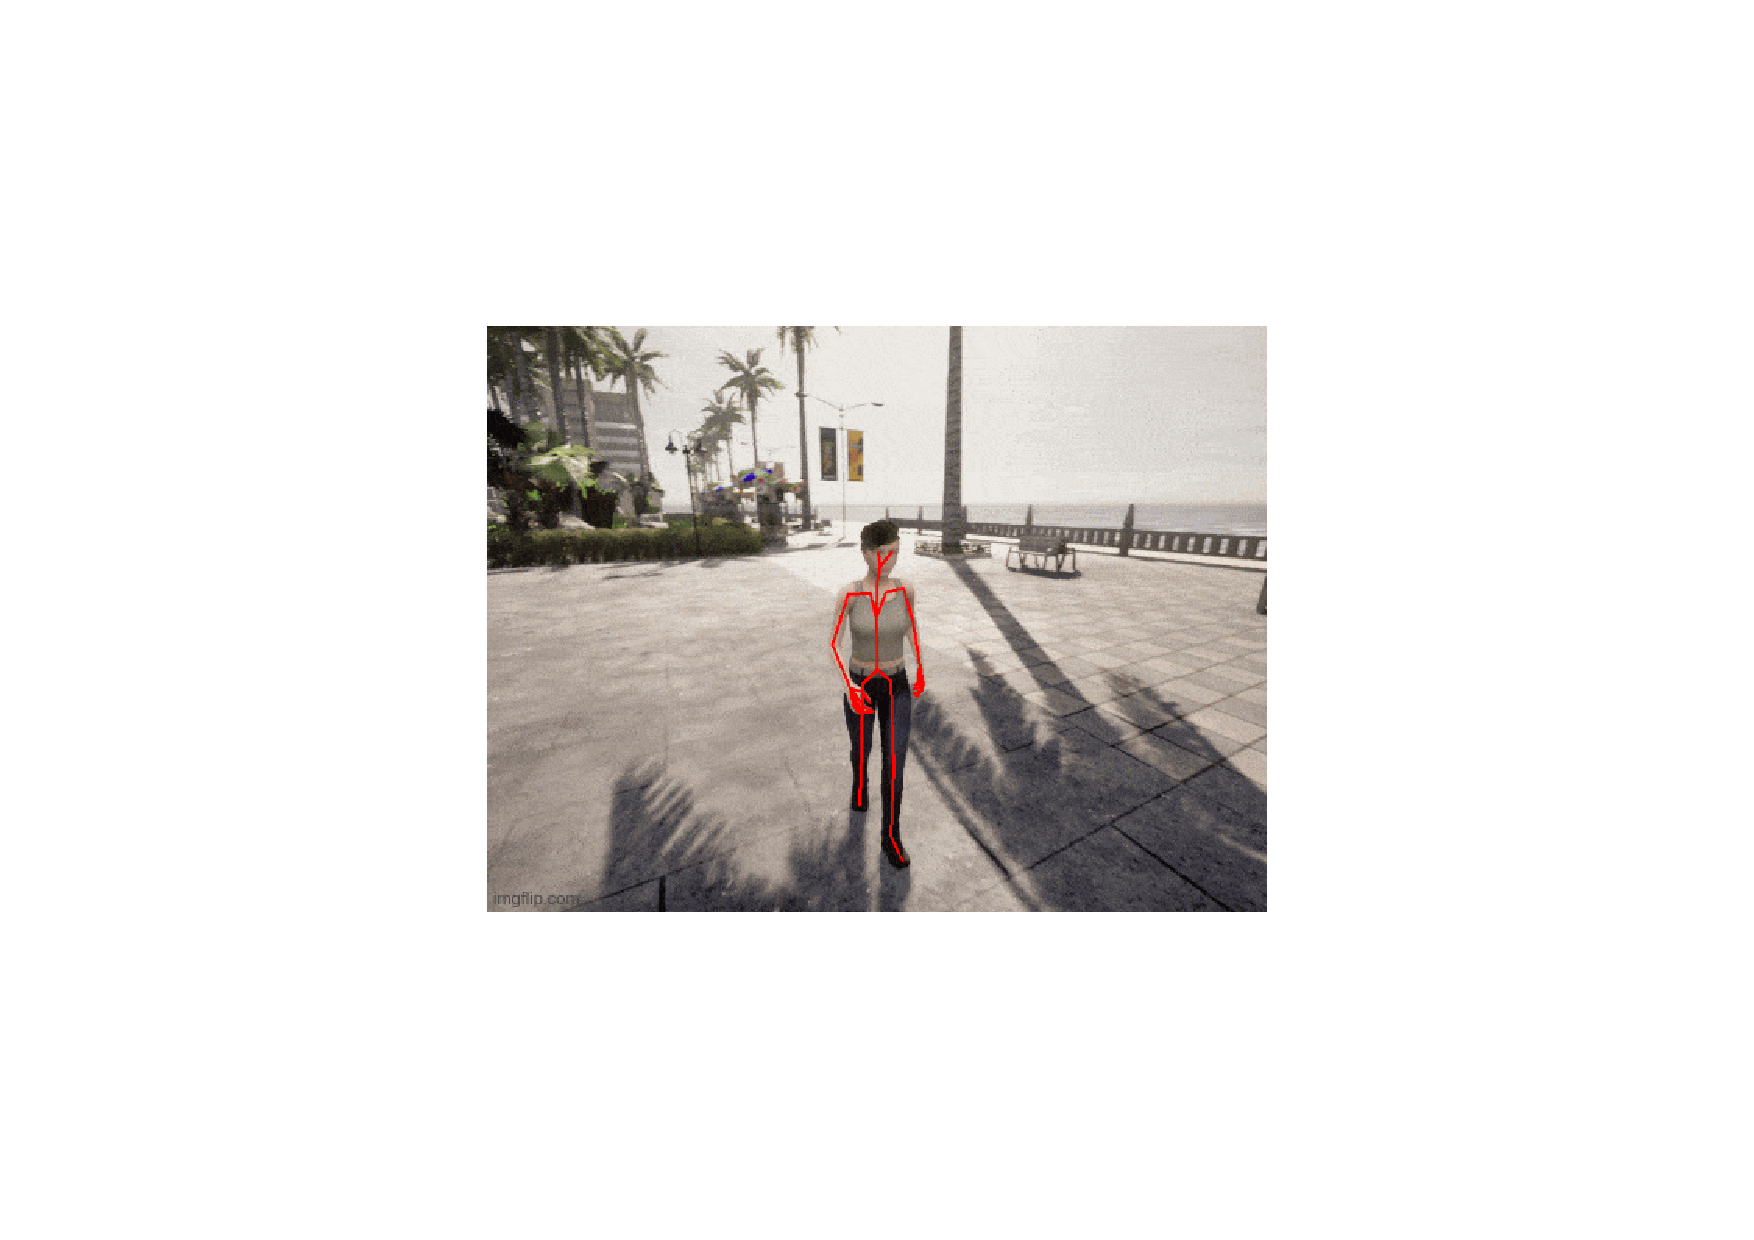
\includegraphics[width=0.8\textwidth]{images/pedestrian_skeleton.pdf}
    \caption{行人骨骼控制示意图}
    \label{fig:pedestrian_skeleton}
\end{figure}

\section{行人行为控制}
本系统行为控制模型基于 Carla 平台 WalkerControl 模块构建,通过设定行人方向和速度参数精确操控移动行为,采用 town5 作为模拟地图,除基本移动功能外支持单向行走与过马路、来回走动两种主要行为模式,这些模式可在不同场景模拟行人多样化行为并满足后续复杂导航任务需求,模块化设计与参数化配置使系统能够灵活适应不同实验需求,为后续深度学习模型在行人避障与导航任务中的集成提供稳定高效的基础环境,初步研究未加入动态障碍物,仅实现行人单独行进,存在一定局限性。

\subsection{单向行走与过马路}
单向行走与过马路是行人基础且关键的行为模式,行人通常从起点出发沿预设路径抵达目标位置,本研究设计简易路线规划系统以精确模拟行人过马路行为,允许其从街道一侧安全移动至对面。如图 \ref{fig:crossing_path},行人从人行道的右侧走向人行道的左侧。

实现时通过设定明确目标位置使行人沿起点到终点的预定路径行走,核心是利用 Carla 平台 WalkerControl 组件设定行人位置、速度等运动参数,该模型作为初步探索 Carla 行人行为模拟的实践较为简单。

\begin{figure}[H]
    \centering
    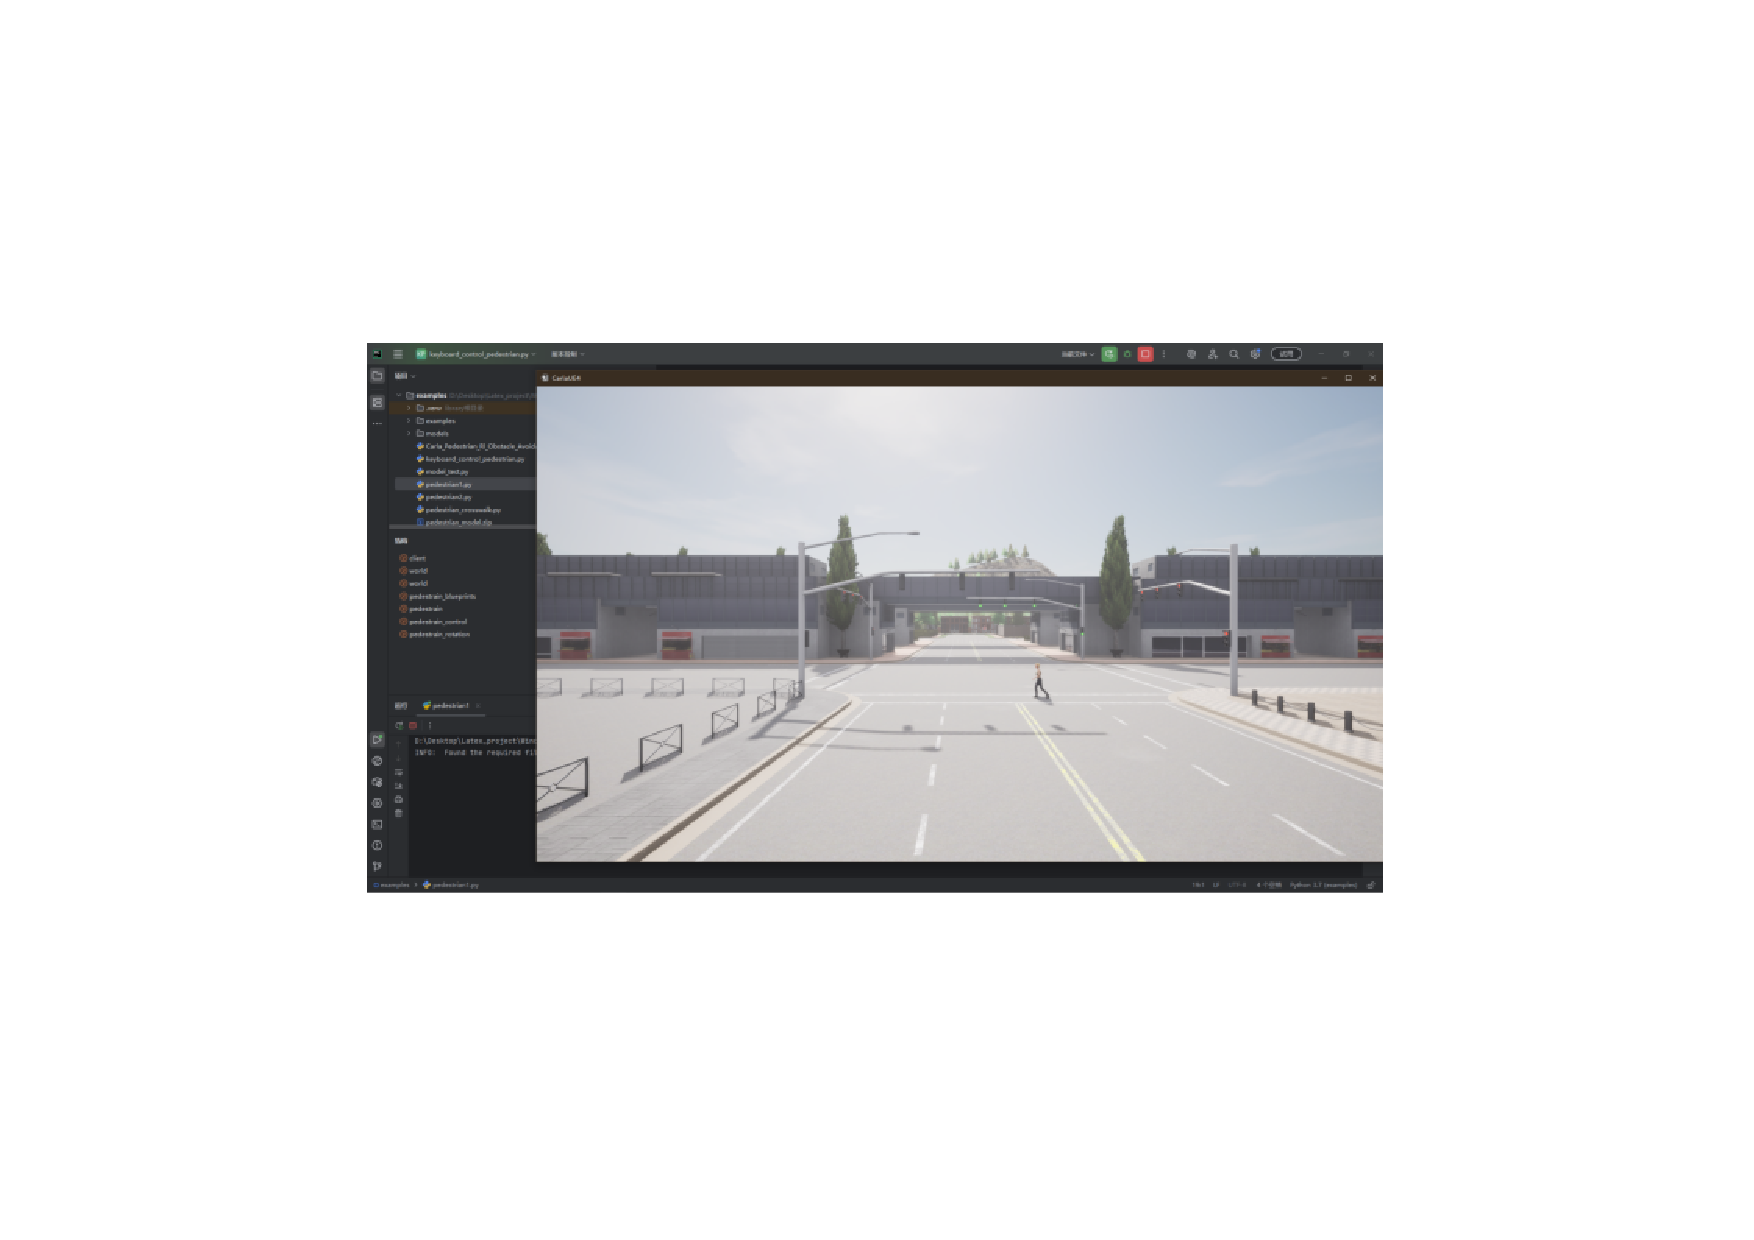
\includegraphics[width=0.8\textwidth]{images/crossing_path.pdf}
    \caption{行人单向行走与过马路示意图}
    \label{fig:crossing_path}
\end{figure}

\subsection{来回走与路径控制}
来回走动是行人在两个固定点间循环往复的常见行走模式,适用于短距离反复行走场景如本次模拟的过马路过程,其实现通过设定目标点并实时更新目标位置确保行人按既定路径高效移动。如图 \ref{fig:walking_back_and_forth},行人到达人行道一侧以后开始转向,向另一侧行进。

实现时先指定两个目标位置,行人到达一个目标后系统自动切换目标使其返回起点,该过程可完全自动化或根据需求允许手动控制,为应对突发情况系统实时监测环境调整行人动作,如遇红灯原地等候、绿灯直接通行,动态路径调整功能确保行人依实际情况及时反应顺利到达下一个目标,这种智能路径规划技术既提高行走效率和安全性,也为后续导航系统设定目标位置奠定基础。

\begin{figure}[H]
    \centering
    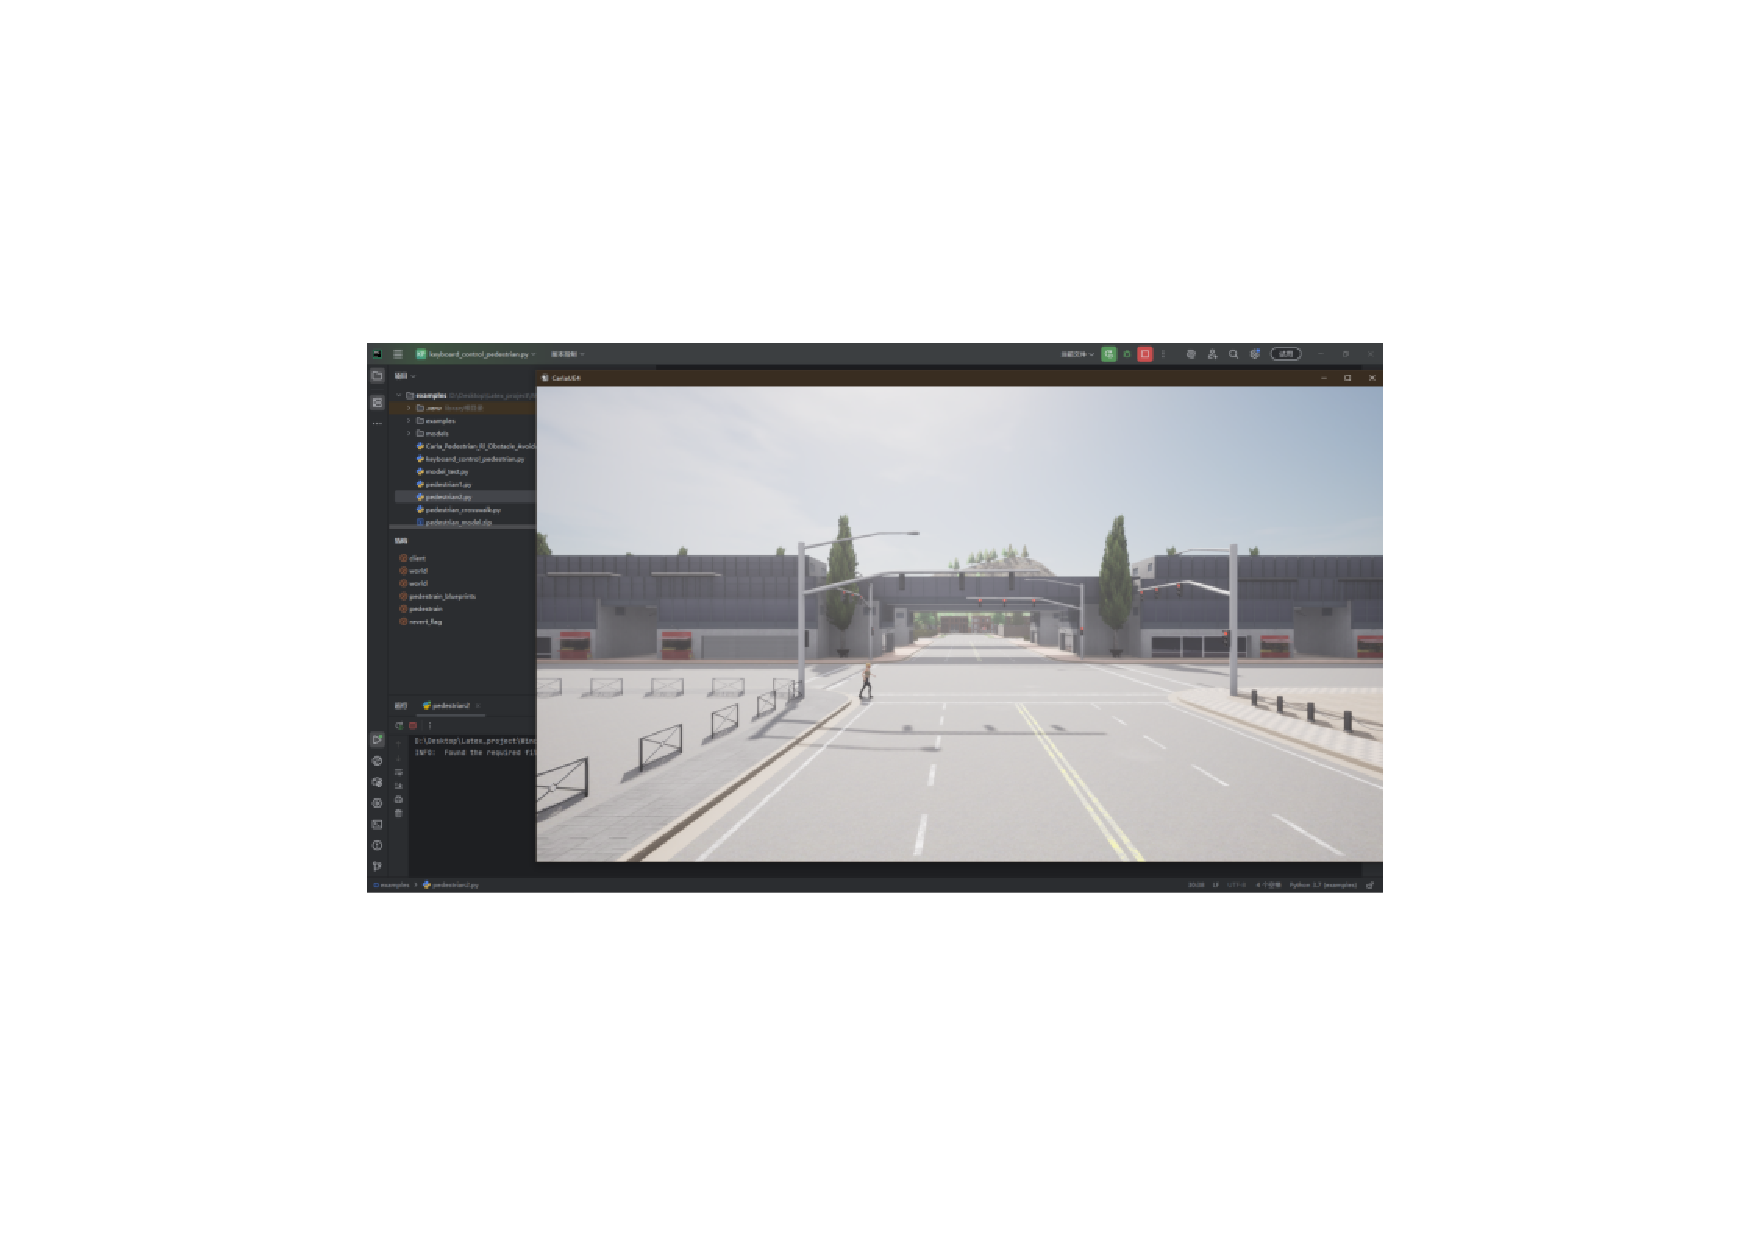
\includegraphics[width=0.8\textwidth]{images/walking_back_and_forth.pdf}
    \caption{行人来回走行为与来回过马路示意图}
    \label{fig:walking_back_and_forth}
\end{figure}

\section{键盘控制行人移动}
本研究设计并实现键盘控制功能以提升用户体验和系统互动性,用户可通过简单键盘输入直接操控行人运动,采用 Pygame 库监听键盘输入,支持按下 W、A、S、D 键实现前进、后退、转向等动作控制,同时在 Pygame 可视化框中提供障碍物识别和监测功能,遇障碍物时屏幕显示距离等实时反馈,如图 \ref{fig:collision_detection},此时屏幕上会显示出障碍物的距离以及相关警告,相关训练代码在地图 town1 中实现。

\begin{figure}[H]
    \centering
    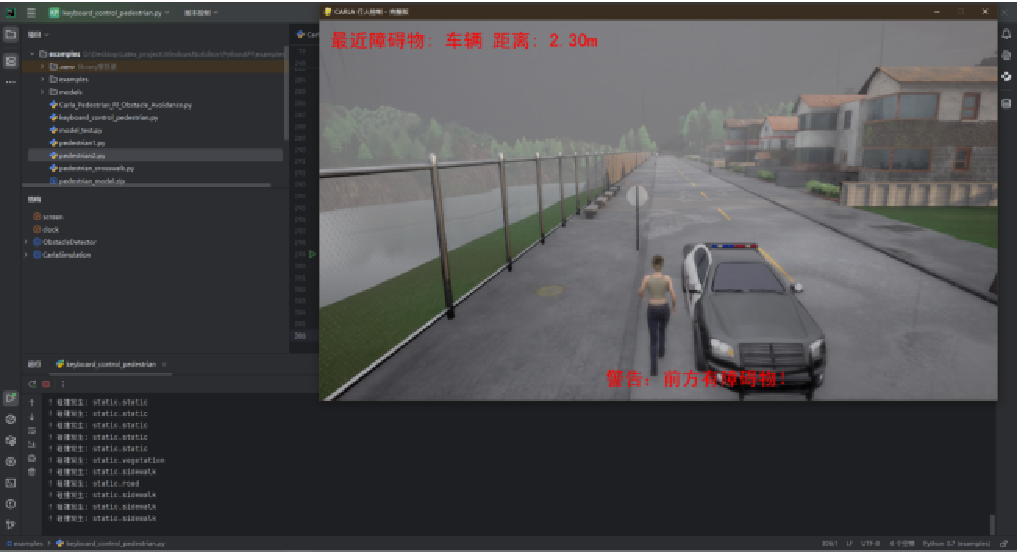
\includegraphics[width=0.8\textwidth]{images/collision_detection.pdf}
    \caption{行人障碍物检测示意图}
    \label{fig:collision_detection}
\end{figure}

具体实现过程包含以下步骤:通过 Pygame 库设置键盘事件监听功能使系统捕捉用户键盘操作并与行人运动方向精确映射,具体规则如图 \ref{fig:keyboard_control}所示,确保用户键盘输入的每一指令被系统准确识别执行;设计控制逻辑使用户输入指令后行人的 WalkerControl 模块实时响应,根据指令更新行人方向和速度,确保行人移动即时准确反映用户控制意图以实现精确控制;考虑行人运动安全性,系统加入碰撞检测与停止机制,当行人遇障碍物时内置碰撞传感器立即检测并触发碰撞事件,系统接收到事件后迅速反应停止行人运动,有效避免碰撞风险保障行人运动安全性。

\begin{figure}[H]
    \centering
    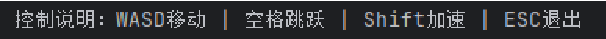
\includegraphics[width=0.8\textwidth]{images/keyboard_control.pdf}
    \caption{键盘控制行人规则}
    \label{fig:keyboard_control}
\end{figure}

键盘控制模块不仅能实现对行人的灵活操控,也为调试与实验分析提供了完善的交互与可视化支持,为后续引入 AI 控制与自动化策略奠定基础。
